\documentclass[main.tex]{subfiles}

\begin{document}
\sloppy


\vspace{1.0cm}

\section{Redesign gerarchia dei FixtureComponent}\label{sec:FixtureComponentHierachy}
I FixtureComponent formano uno strato che si pone tra i dati DMX che arrivano ad UnrealEngine ed i materiali visti nel capitolo precedente. Mentre i materiali Light/Lens/Beam definiscono come effettuare il rendering della luce emessa da un faro, i FixtureComponent ne controllano i comportamenti e comunicano con i primi attraverso i parametri presenti nei vari moduli della pipeline che abbiamo creato in precedenza. Un altro modo che i FixtureComponent hanno per interagire con un faro istanziato in un mondo virtuale è andando direttamente a modificarne le proprietà (Ad esempio la rotazione delle varie geometrie). \newline

In questo capitolo analizzeremo i problemi riscontrati nell'implementazione di un nuovo componente e proporremo una nuova gerarchia atta all'aggiunta di nuove features nella maniera più semplice possibile.

\subsection{Vecchia implementazione}\label{subsec:3_oldImplementation}
I FixtureComponent sono, realmente, delle classi organizzate in una struttura gerarchica. Alla base abbiamo \lstinline{FixtureComponentBase}, esteso da \lstinline{SimpleAttributeFixtureComponent} (Ovvero singole features che vengono controllate in maniera diretta) e da \lstinline{MultipleAttributeFixtureComponent} (Ovvero features che vengono controllate da più canali, oppure che possono avere comportamenti avanzati).
\begin{figure}[H]
    \centering
    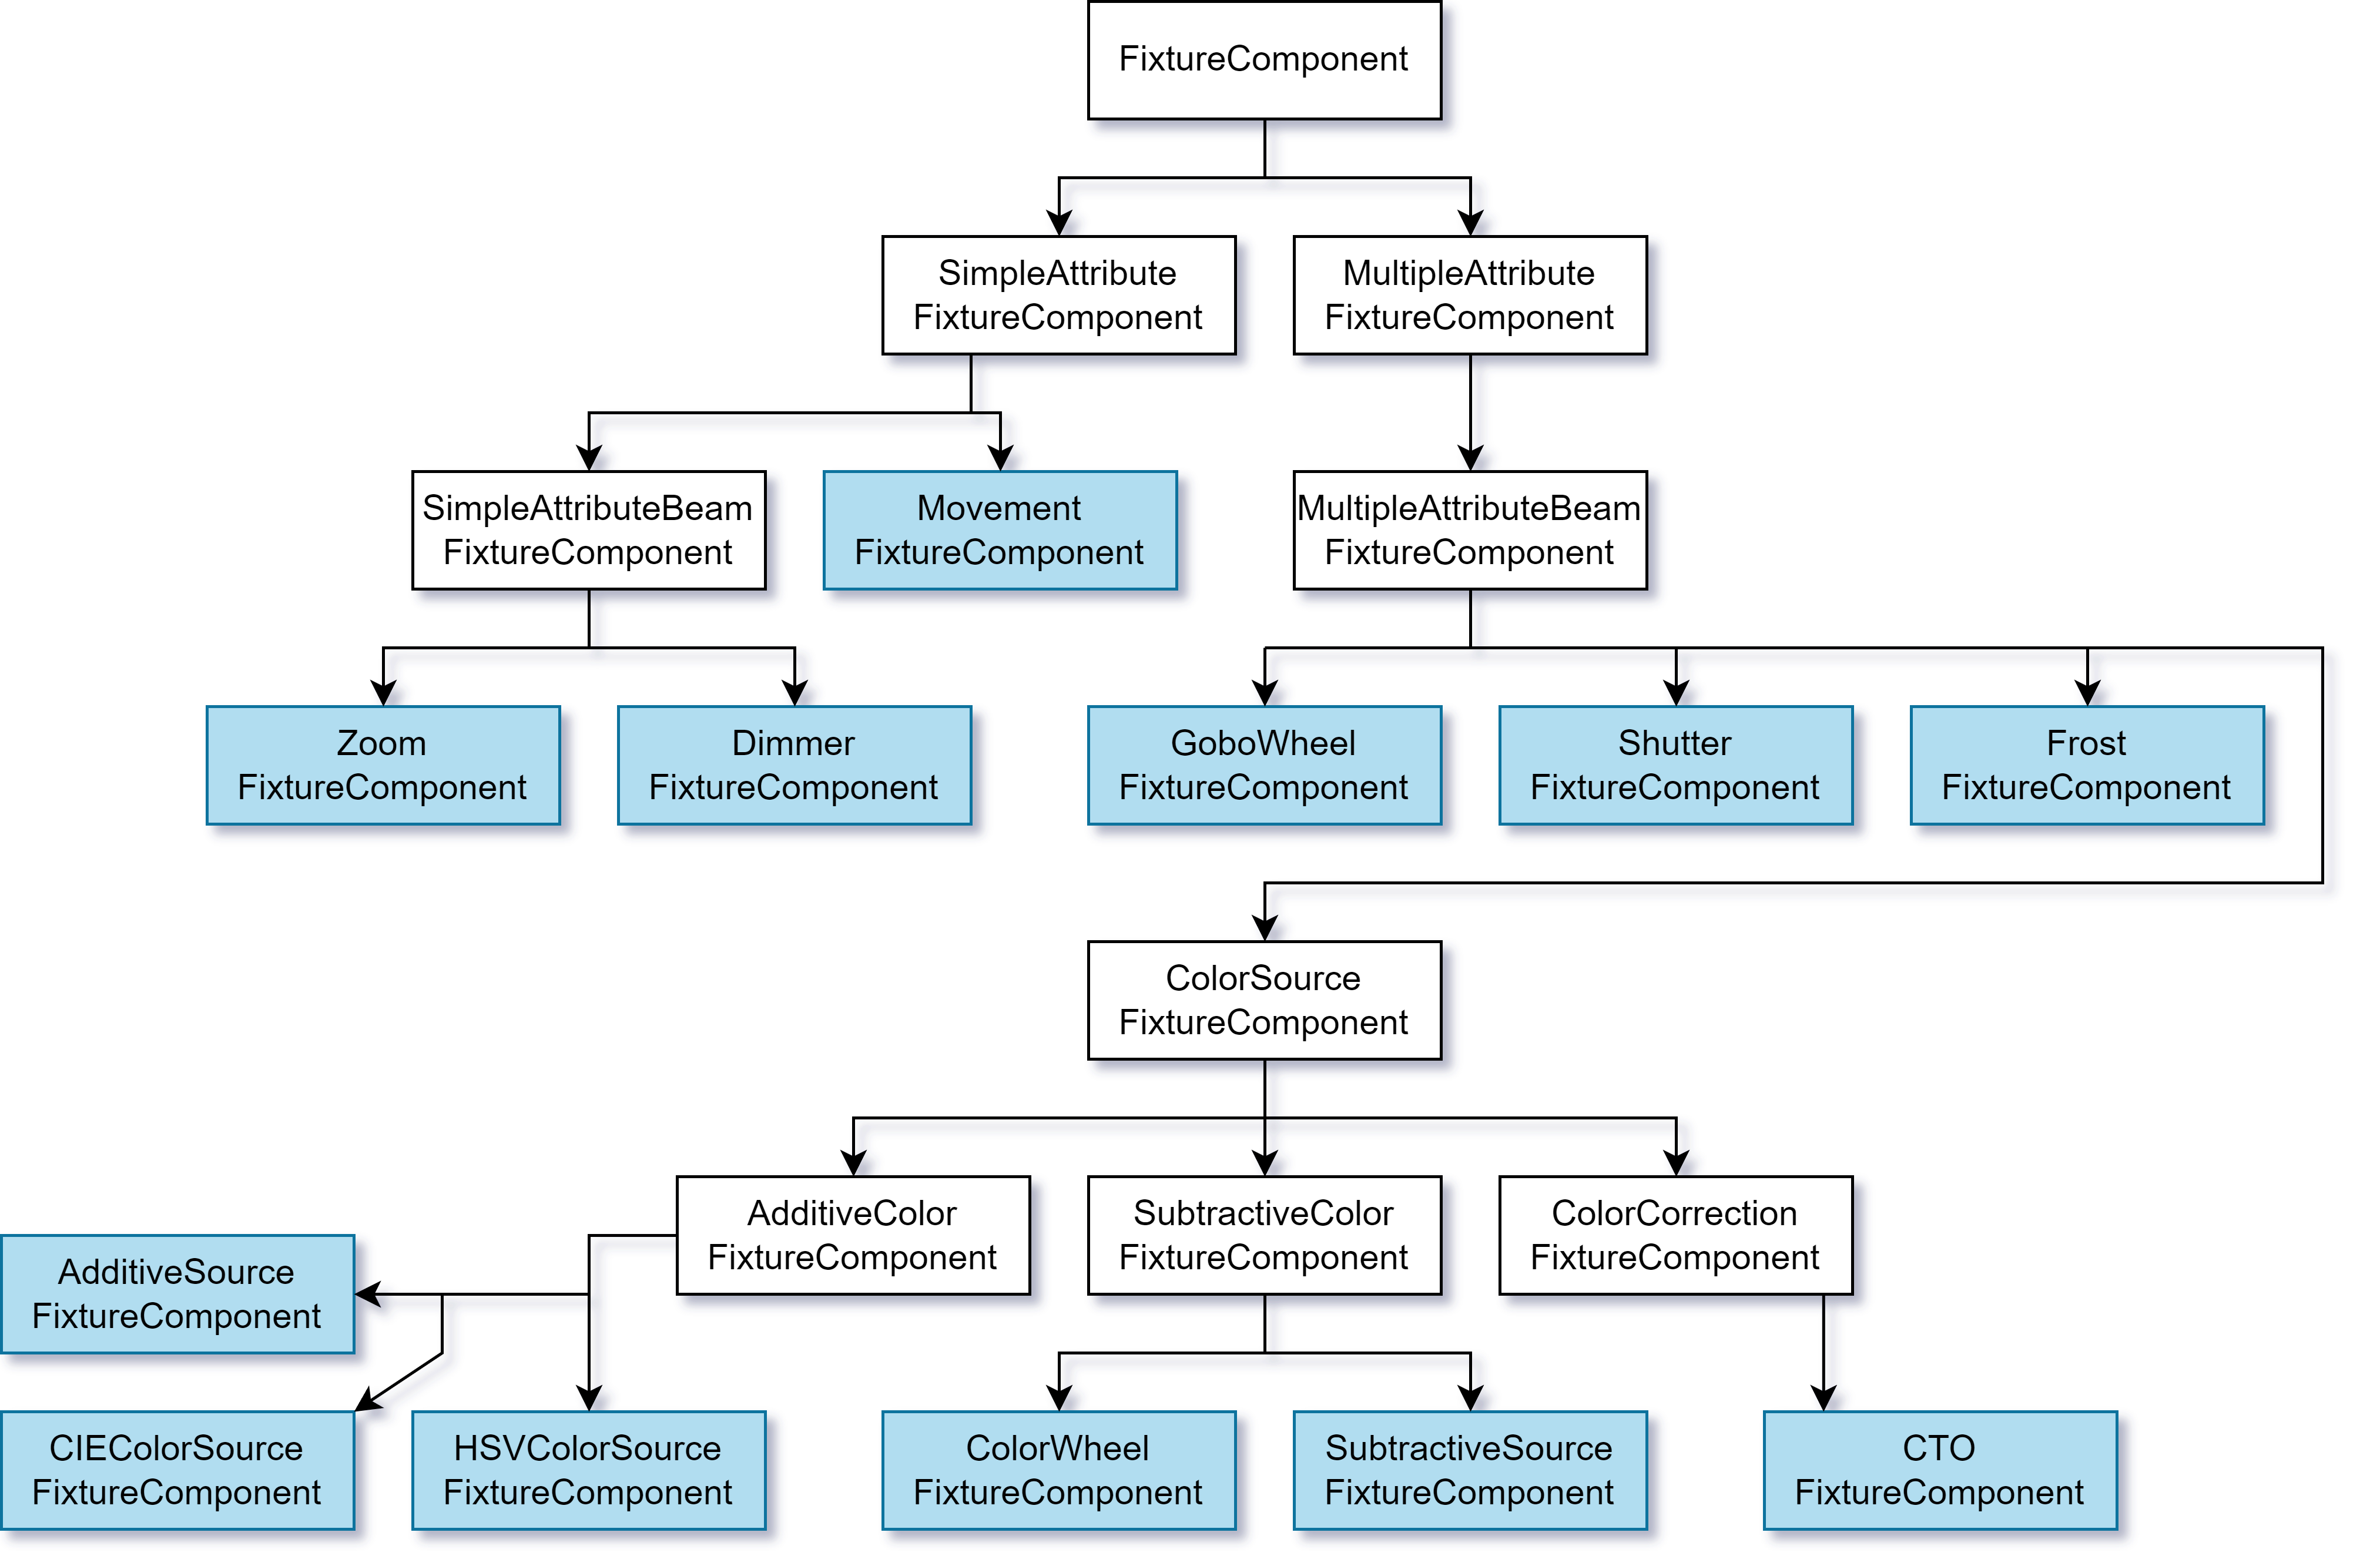
\includegraphics[width=0.9\linewidth]{img/fixtureComponent/FixtureComponentOLD.drawio.png}
    \caption{Struttura gerarchica delle classi FixtureComponent. In azzurro i componenti veri e propri.}
    \label{fig:3_fixtureComponentOld}
\end{figure}

I FixtureComponent vengono istanziati dalla classe \lstinline{FCPFActorComponentsLoader}, che si occupa anche di richiamare \lstinline{Setup()}. Setup è un metodo che viene essenzialmente duplicato in ogni componente e che si occupa di salvarsi il DMXChannel in cui il componente è presente, costruire un albero di LogicalChannel, salvarsi la geometria a cui si fa riferimento e ottenere il Canale DMX in cui è presente il componente. Quando una fixture istanziata in un mondo inizia ad essere emulata, viene chiamato \lstinline{BeginPlay()} su ogni suo componente che, attraverso del codice parzialmente duplicato, inizializzerà di nuovo l'albero dei LogicalChannel e inizializzerà l'interpolazione con dei valori hard-coded. A questo punto la fixture sarà \say{in esecuzione} e risponderà a due tipi di eventi:
\begin{itemize}
    \item \textbf{Nuovo pacchetto DMX}: Ogni volta che arriva un nuovo pacchetto DMX viene chiamata la funzione \lstinline{PushNormalizedRawValues} (implementata dentro \lstinline{FixtureComponentBase}) che chiama a sua volta \lstinline{PushDMXRawValues}. Quest'ultima funzione è implementata allo stesso identico modo su ogni singolo componente. Quello che fa è chiamare \lstinline{ApplyEffectToBeam} con il valore dmx del canale. Se un componente gestisce riceve input da più DMXChannel, ci sarà una chiamata hard-coded (senza alcun ciclo for) per ciascuno. \lstinline{ApplyEffectToBeam} si occupa di interpretare i dati in arrivo. L'output di questo processo viene effettuato attraverso 3 funzioni: \lstinline{SetTargetValue}, \lstinline{SetValueNoInterp} e \lstinline{interp.SetValueNoInterp}.
    \item \textbf{È scorso un nuovo tick}: Viene chiamata \lstinline{InterpolateComponent} che viene rimplementata da ogni componente ed in ciascuno si occupa di aggiornare lo stato interno degli effetti delle feature (Esempio: FrostPulseOpen) controllate dallo stesso, utilizzando anche qui le funzioni \lstinline{SetTargetValue}, \lstinline{SetValueNoInterp} e \lstinline{interp.SetValueNoInterp}. Successivamente aggiorna lo stato dell'interpolazione.
\end{itemize}
\lstinline{SetTargetValue} è una funzione, attualmente rimplementata in maniera identica da tutti i componenti, che serve ad impostare un nuovo valore di destinazione all'interpolazione. Prima di impostare un nuovo target, controlla se l'interpolazione è attiva e se è già stato impostato un primo valore. In caso negativo, viene chiamata direttamente la funzione \lstinline{SetValueNoInterp}, implementata dentro \lstinline{MultipleAttributeBeamFixtureComponent}, che si occupa di chiamare \lstinline{SetValueNoInterp_BeamInternal} con un for su ogni geometria, che a sua volta si occupa di mandare in output verso i materiali i valori elaborati dal componente.
\lstinline{interp.SetValueNoInterp} è una funzione dell'oggetto interpolazione che lo fa saltare direttamente a quel valore.

\begin{figure}[H]
    \centering
    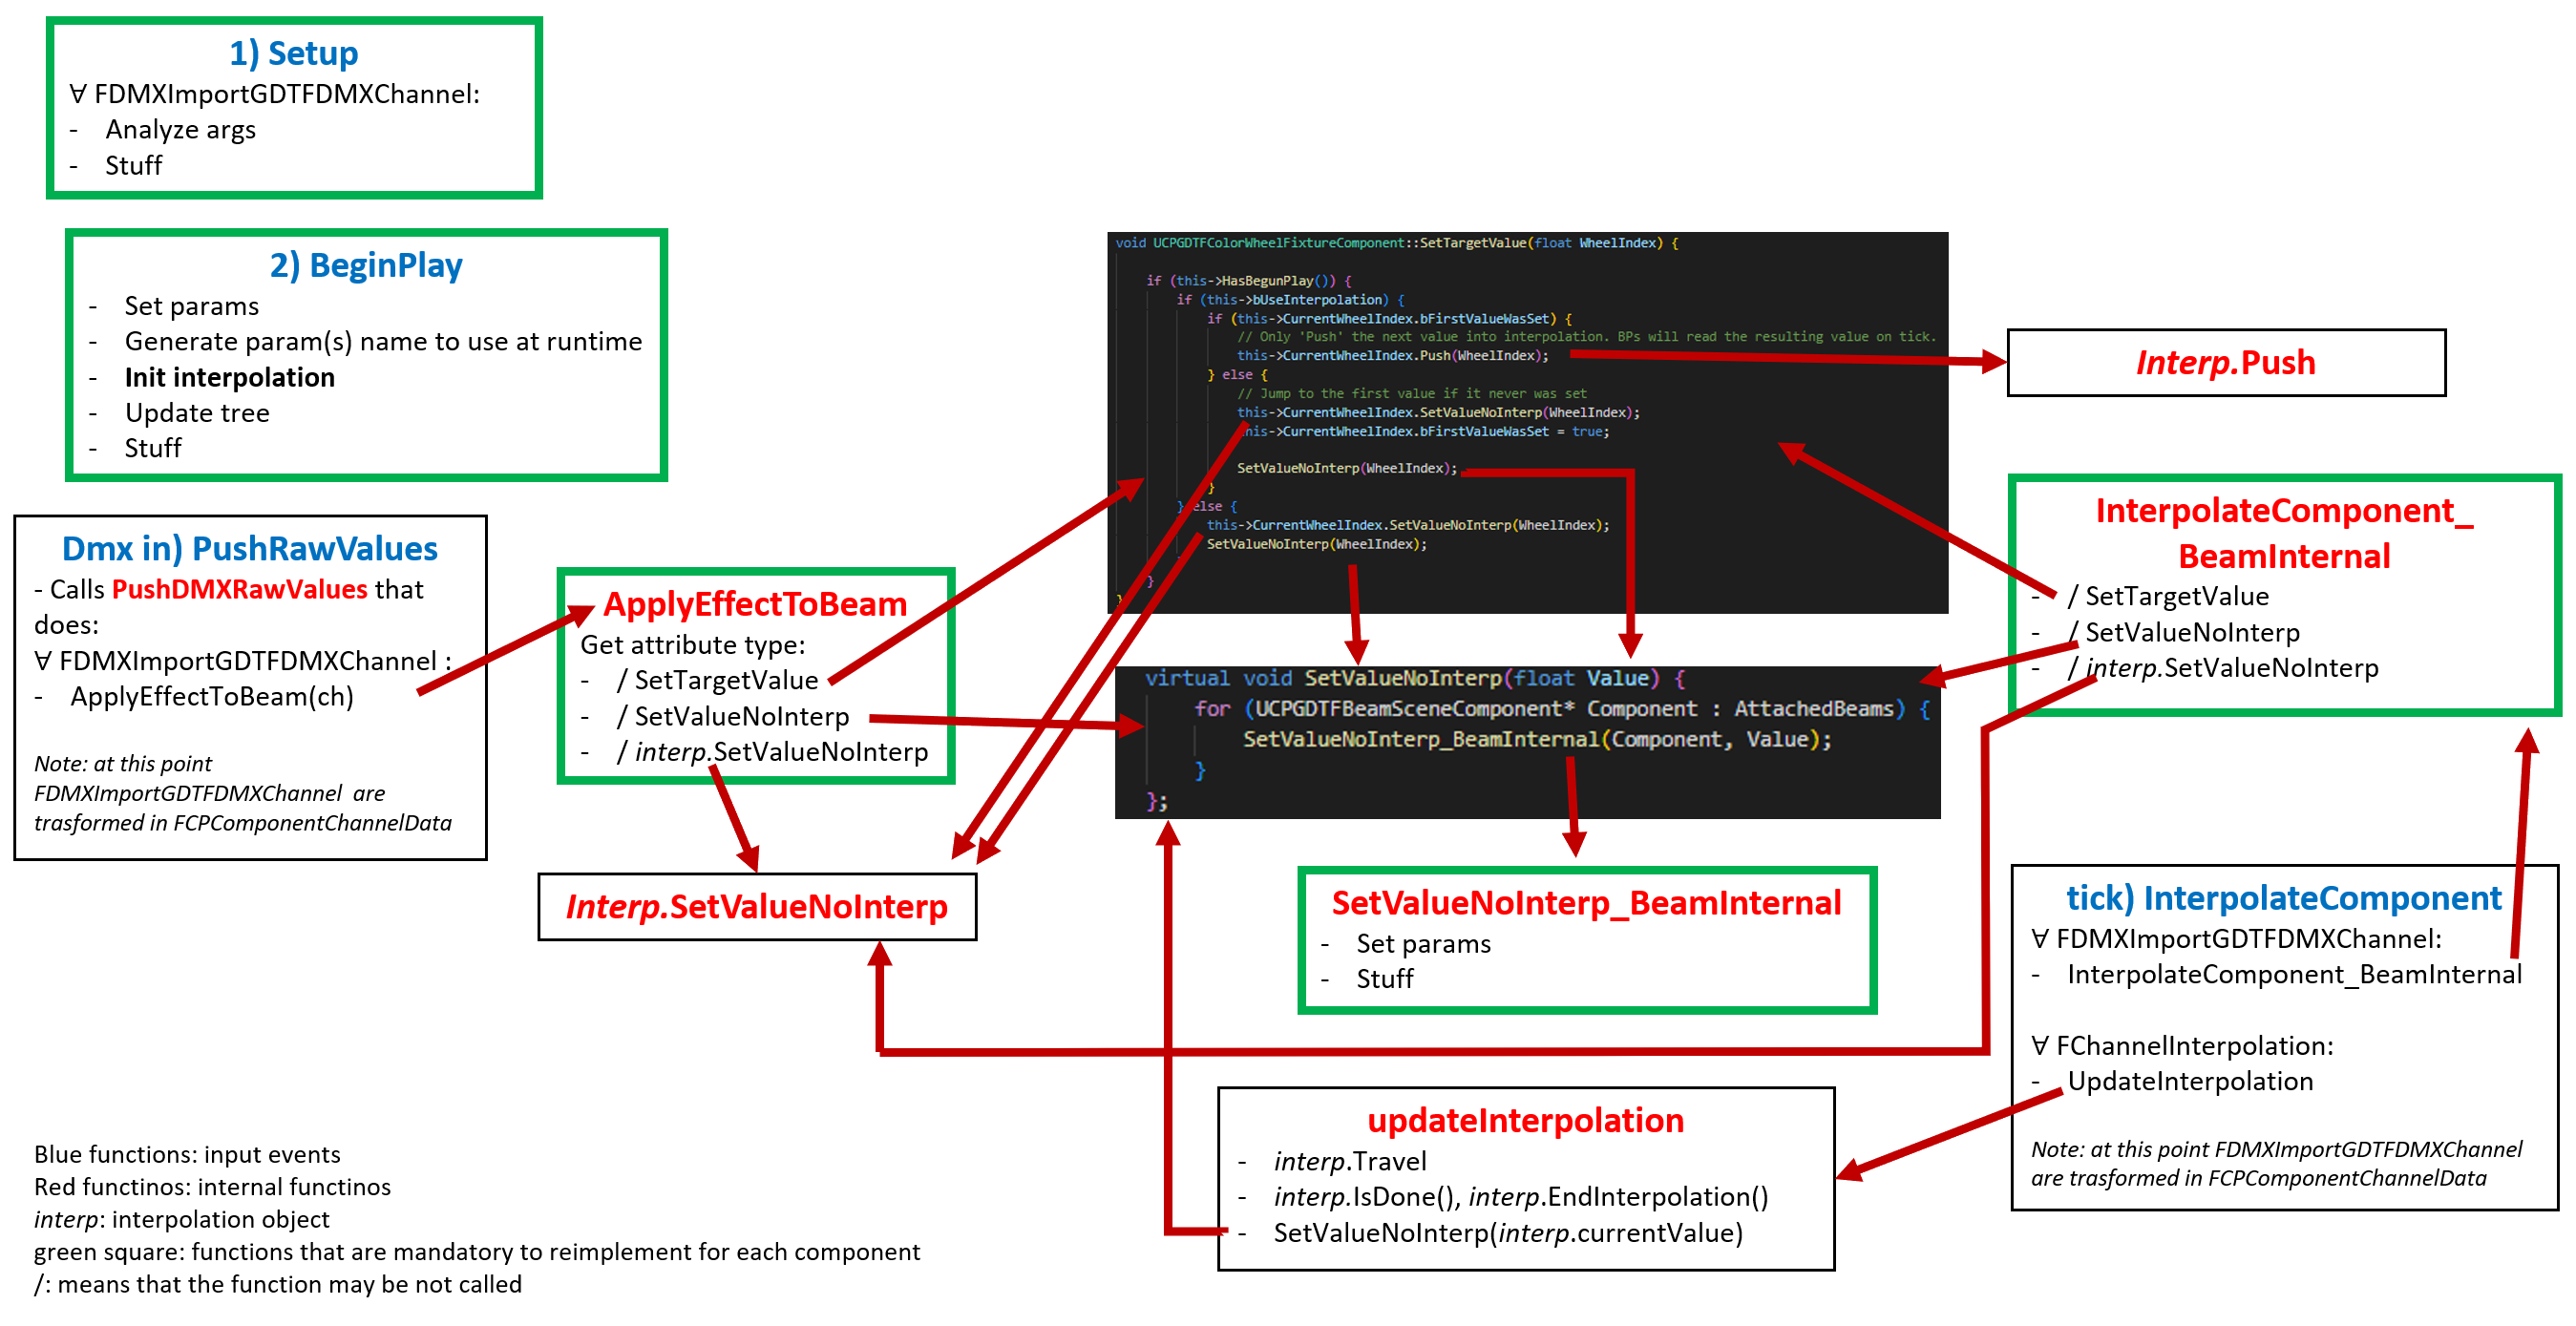
\includegraphics[width=1\linewidth]{img/fixtureComponent/CallOrderScheme.png}
    \caption{Schema creato in corso d'opera mentre svolgevo reverse-engineering sulla vecchia implementazione dei FixtureComponent. Le funzioni in azzurro sono triggerate da eventi esterni, quelle in rosso sono le funzioni interne. I quadrati verdi sono gli unici che, in una implementazione ideale, dovrebbero essere specializzati da ogni singolo componente.}
    \label{fig:3_CallOrderOld}
\end{figure}

Analizzando l'implementazione di questa gerarchia sono sorte delle criticità:
\begin{itemize}
    \item \textbf{Codice duplicato}: Nonostante alcune funzioni siano state dichiarate (come virtuali) in una classe padre, molte classi figlie le reimplementano in maniera identica l'una dall'altra. Un esempio è la funzione \lstinline{} che viene definita nello stesso identico modo da tutti i figli diretti di \lstinline{MultipleAttributeFixtureComponent}:
\lstset{language=UEcpp}
\begin{lstlisting}
void UCPGDTFFrostFixtureComponent::PushDMXRawValues(
        UDMXEntityFixturePatch* FixturePatch,
        const TMap<int32, int32>& RawValuesMap) {

	int32* DMXValuePtr = RawValuesMap.Find(this->ChannelAddress);
	if (DMXValuePtr) this->ApplyEffectToBeam(*DMXValuePtr);
}

void UCPGDTFShutterFixtureComponent::PushDMXRawValues(
        UDMXEntityFixturePatch* FixturePatch,
        const TMap<int32, int32>& RawValuesMap) {

	int32* DMXValuePtr = RawValuesMap.Find(this->ChannelAddress);
	if (DMXValuePtr) this->ApplyEffectToBeam(*DMXValuePtr);
}
\end{lstlisting}
    \item \textbf{Virtualizzazione delle funzioni quasi assente}: Molte funzioni sono presenti su vari componenti della gerarchia, ma non sono mai dichiarate su una classe padre, nonostante facciano la stessa cosa ed è giusto che siano esposte agli altri componenti. Un esempio sono \lstinline{ApplyEffectToBeam} e \lstinline{SetTargetValue} che sono implementate da molti componenti, ma mai definiti in un padre (E sono anche un altro esempio di codice completamente duplicato) 
    \item \textbf{Elementi superflui nella gerarchia}: Elementi come Simple o Multiple AttributeBeamFixtureComponent sono essenzialmente vuoti e non portano miglioramenti alla definizione implicita della gerarchia %TODO CHIEDERE A DAVIDE COME SCRIVERE
    \item \textbf{Nessuna centralizzazione della gestione delle features}: La gerarchia viene definita attraverso delle classi che di fatto sono quasi delle interfacce. Questo comporta che la gestione di tutto che ci sta attorno ad una feature è a carico dei singoli componenti finali. Ogni volta che si implementa un nuovo componente si è quindi obbligati a rimplementare tutta la logica che sta dietro la gestione degli stessi.
    \item \textbf{Bassa chiarezza su cosa deve essere implementato nella singola feature}: Visti i punti precedenti, se si vuole implementare un nuovo componente (senza avere conoscenze pregresse) si rimane interdetti poiché non si capisce esattamente cosa bisogna fare per la realizzazione dello stesso. Non è presente una lista ben definita di funzionalità in cui il singolo componente deve specializzarsi.
    \item \textbf{Errori veri e propri nel calcolo di valori utili}: In generale, sono state riscontrate grosse mancanze con il calcolo di valori utili ad un componente. Ad esempio, il valore di minimo e massimo di una ChannelFunction viene calcolato solamente su quella corrente, piuttosto di avere un valore globale per tutti gli attributi dello stesso tipo. Oppure, i valori di fade e accelerazione per l'interpolazione non venivano proprio calcolati né presi dal GDTF originale.
    \item \textbf{Interpolazione mancante su molti componenti}: L'interpolazione non è gestita nella maniera corretta, di conseguenza è completamente mancante su molte feature di un faro (Ad esempio zoom, o rotazione di una gobo). Più specificatamente, è presente solamente sui componenti che estendono \lstinline{MultipleAttributesFixtureComponent} e se uno stesso componente controlla più features è attiva solo su una delle due
    \item \textbf{Gestione di $N > 1$ canali hard-coded}: Se un componente gestisce più features oppure se riceve dati da più DMXChannel, la gestione di ogni singolo viene fatta copiando ed incollando il codice di uno N volte, piuttosto che avere dei for che li scorrono
\end{itemize}

Per risolvere queste criticità è stato deciso un redesign dei vari FixtureComponent. A livello gerarchico non ci saranno molte differenze; esse saranno presenti maggiormente lato implementazione.

\subsection{Idea di reimplementazione}\label{subsec:3_idea}
Idealmente un componente dovrebbe definire pochi comportamenti specializzanti:
\begin{itemize}
    \item Costruttore del componente (in cui, ad esempio, possono essere caricate eventuali texture o altre informazioni).
    \item \lstinline{BeginPlay()} per inizializzare il materiale e fornire i dati per inizializzare le interpolazioni.
    \item Definire gli AttributeGroups, ovvero una lista in cui vengono raggruppati attributi differenti del GDTF che però corrispondono alla stessa funzionalità (ES: \lstinline{Gobo_n_WheelShake} e \lstinline{Gobo_n_PosShake}) e che, materialmente, vengono usati insieme dentro \lstinline{ApplyEffectToBeam()}. Attributi differenti che fanno parte dello stesso AttributeGroup condividono gli stessi valori default/min/max.
    \item Valori default per l'interpolazione, in caso non vengano forniti dal file GDTF.
    \item \lstinline{ApplyEffectToBeam()} per definire come una feature si deve comportare all'arrivo di nuovi valori DMX. Viene automaticamente scorso l'elenco dei canali per cui un componente è in ascolto e la funzione, a differenza di prima, deve ricevere tutte le informazioni del DMXChannel già elaborate, al posto di elaborarle da solo. 
    \item \lstinline{InterpolateComponent_BeamInternal()} per definire come la luce si deve comportare ad ogni tick, se ci sono effetti in esecuzione.
    \item \lstinline{SetValueNoInterp_BeamInternal()} per definire come inviare i dati elaborati dal componente, verso il materiale. A differenza di prima questa funzione dovrà supportare più feature differenti, invece di avere un SetValueNoInterp per ogni feature differente.
\end{itemize}

Tutto il resto invece dovrebbe essere appannaggio \say{automatico} dei padri, principalmente di \lstinline{FixtureComponentBase}
%TODO spiegazione precisa di fcbase

\subsubsection{Strutture dati}\label{subsec:3_2_structs}

\subsection{Implementazione}\label{subsec:3_implementation}
\subsubsection{Ottenimento valori di default per le varie funzionalità di una fixture}\label{subsec:3_1_defaultValues}

\end{document}